\begin{problem}
  Find a positive angle co-terminal with (and not equal to) $\frac{4\pi}{7}$.
  The units of answer should be \textit{radians}.) Provide an exact value.
  \textbf{[$2$ points]}
\end{problem}

\begin{solution}
  The definition of Co-Terminal is:
  \textbf{Two angles with the same terminal side.}

  Now, to get two angles with the same terminal side, you have to add
  $360^{\circ}$ to it. Hence, you need to make the other angle do a full
  rotation around, but still land back in the same spot. Since we have to do
  this in radians, we'll use the following conversion factor: $2\pi =
  360^{\circ}$. Simply enough, add $2\pi$ to $\frac{4\pi}{7}$, and that will be
  your co-terminal angle:

  \begin{align*}
    \frac{4\pi}{7} + 2\pi &= \frac{4\pi}{7} + \frac{2\pi}{1} \\
      &= \frac{4\pi}{7} + \frac{14\pi}{7} \\
      &= \boxed{\frac{18\pi}{7}}
  .\end{align*}

  So, here are your co-terminal angles:

  \begin{align*}
    \frac{4\pi}{7} \qquad \frac{18\pi}{7}
  .\end{align*}
\end{solution}

\newpage

\begin{problem}
  Find a negative angle co-terminal with (and not equal to) $85^{\circ}$. (The
  units if your answer should be \textit{degrees}.) Provide an exact value.
  \textbf{[$2$ points]}
\end{problem}

\begin{solution}
  To find a negative co-terminal angle, we subtract $360^{\circ}$ because a
  co-terminal angle are two angles that share the same terminal side.

  \[ 85^{\circ} - 360^{\circ} = \boxed{- 275^{\circ}} \].
\end{solution}

\newpage

\begin{problem}
  In the table below, some angles are given in both degrees and radians.
  Complete the table by filling in the six missing values. You don't need to
  show any work. \textbf{[$3$ points]}

  \begin{table}[H]
    \label{tab:degrees_into_radians}
    \centering

    \begin{tabular}{|c|c|c|c|c|c|c|c|c|}
      \hline
      $\theta$ (degrees) & $0^{\circ}$ & $30^{\circ}$ & $$ & $60^{\circ}$ & $$ & $270^{\circ}$ & $$ & $360^{\circ}$ \\
      \hline
      $\theta$ (radians) & $0$ & $$ & $\frac{\pi}{4}$ & $$ & $\frac{4\pi}{3}$ & $$ & $\frac{11\pi}{6}$ & $2\pi$ \\
      \hline
    \end{tabular}

    \caption{Degrees into Radians}
  \end{table}
\end{problem}

\begin{solution}
  \begin{table}[H]
    \label{tab:degrees_into_radians}
    \centering

    \begin{tabular}{|c|c|c|c|c|c|c|c|c|}
      \hline
      $\theta$ (degrees) & $0^{\circ}$ & $30^{\circ}$ & $45^{\circ}$ & $60^{\circ}$ & $240^{\circ}$ & $270^{\circ}$ & $330^{\circ}$ & $360^{\circ}$ \\
      \hline
      $\theta$ (radians) & $0$ & $\frac{\pi}{6}$ & $\frac{\pi}{4}$ & $\frac{\pi}{3}$ & $\frac{4\pi}{3}$ & $\frac{3\pi}{2}$ & $\frac{11\pi}{6}$ & $2\pi$ \\
      \hline
    \end{tabular}

    \caption{Common Values for Sin and Cos}
  \end{table}
\end{solution}

\newpage

\begin{problem}
  Convert the angle $\frac{2\pi}{5}$ (in radians) into degrees. Provide an exact
  value. \textbf{[$2$ points]}
\end{problem}

\begin{solution}
  To do this, we need a conversion factor. I'm going to use: $\pi =
  180^{\circ}$:

  \begin{align*}
    \frac{2\pi}{5} \times \frac{180^{\circ}}{\pi} &= \frac{2}{5} \times 180^{\circ} \\
      &= \frac{2 \times 180^{\circ}}{5} \\
      &= \boxed{72^{\circ}}
  .\end{align*}
\end{solution}

\newpage

\begin{problem}
  What is the length of the arc spanned by an angle of $36^{\circ}$ in a circle
  of radius $15$ feet? Provide an exact value. \textbf{[$3$ points]}
\end{problem}

\begin{solution}
  To answer this problem, we need to convert the degrees into radians first:

  \begin{align*}
    36^{\circ} \times \frac{\pi}{180^{\circ}} &= \frac{\pi}{5} \textrm{ rad}
  .\end{align*}

  Now, we can use the formula:

  \begin{align*}
    s &= r \times \mid \theta \mid \\
      &= 15 \times \frac{\pi}{5} \\
      &= \boxed{3\pi}
  .\end{align*}
\end{solution}

\newpage

\begin{problem}
  List the period, midline, and amplitude of the function $y = g(t)$. Note that
  the following points are on the graph:
  $\left(-\frac{\pi}{4}, 2\right), \left(\frac{\pi}{12}, -10\right),
  \left(\frac{5\pi}{12}, 2\right)$ and $\left(\frac{3\pi}{4}, -10\right)$.
  \textbf{[$3$ points]}
\end{problem}

\begin{figure}[H]
  \centering
  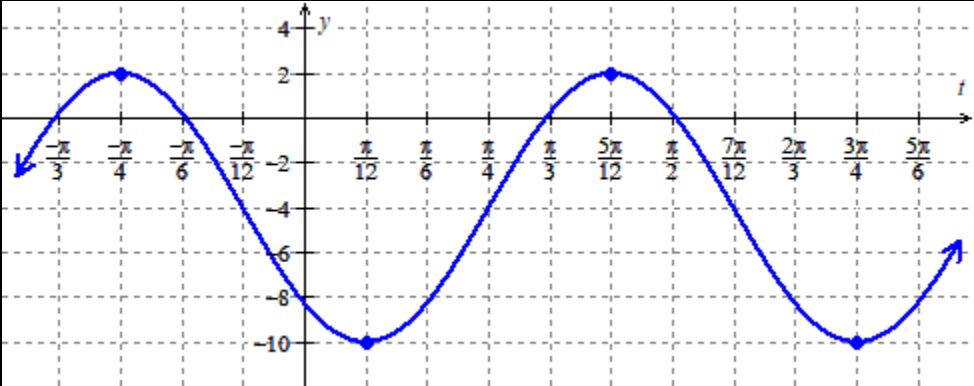
\includegraphics[width=0.8\textwidth]{images/week-1.png}
  \caption{}
  \label{fig:week_1}
\end{figure}

\begin{solution}
  \subsection*{Period}
  \label{sub_sec:period}

  I like to think of the period as the distance between either the maximum value
  and the minimum value. So, just subtract the maximum value from the one next
  to it, or do it with the minimum value. (I'm using the maximum):

  \begin{align*}
    \frac{5\pi}{12} - (-\frac{\pi}{4}) = \frac{2\pi}{3}
  .\end{align*}

  % subsection period (end)

  \subsection*{Midline}
  \label{sub_sec:midline}

  The formula for finding the midline is:

  \begin{align*}
    y &= \frac{f_{\textrm{max}} + f_{\textrm{min}}}{2} \\
      &= \frac{2 + (-10)}{2} \\
      &= \frac{8}{2} \\
      &= \boxed{4} \\
  .\end{align*}

  % subsection midline (end)

  \subsection*{Amplitude}
  \label{sub_sec:amplitude}

  The amplitude is the distance between the maximum value and the midline value or the
  function's minimum value and the midline value.

  From the graph, we can see that it takes \boxed{$6 \textrm{units}$} to go from the
  minimum and maximum value to the midline.

  % subsection amplitude (end)
\end{solution}
